\chapter{Методы исследования} \label{methods}

\section{Математическая формализация проблемы инвариантности}
\label{methods:math}

\subsection{Проблема алиасинга в CNN}
\label{methods:math:aliasing}

С точки зрения теории обработки сигналов, операции даунсэмплинга в CNN могут приводить к алиасингу, что является основной причиной нарушения инвариантности к сдвигам. Рассмотрим математическую формализацию этой проблемы.

Пусть $\mathbf{x}$ — входное изображение, а $T_{\delta}\mathbf{x}$ — то же изображение, сдвинутое на вектор $\delta$. В идеальном случае, функция извлечения признаков $f$ должна быть эквивариантна к сдвигам, то есть:

\begin{equation}
f(T_{\delta}\mathbf{x}) = T_{\delta}f(\mathbf{x})
\end{equation}

Однако в реальности операции даунсэмплинга нарушают это свойство. Рассмотрим операцию субдискретизации с шагом 2, которая может быть представлена как:

\begin{equation}
(S_2 \mathbf{x})[n] = \mathbf{x}[2n]
\end{equation}

Такая операция не коммутирует с оператором сдвига. Например, для сдвига на 1 пиксель:

\begin{equation}
S_2(T_1 \mathbf{x})[n] = (T_1 \mathbf{x})[2n] = \mathbf{x}[2n+1]
\end{equation}

\begin{equation}
T_{1/2}(S_2 \mathbf{x})[n] = (S_2 \mathbf{x})[n+1/2] \approx \mathbf{x}[2n+1]
\end{equation}

Это несоответствие является источником нестабильности активаций и выходных предсказаний при субпиксельных сдвигах входных данных.

\section{Модификации архитектур с анти-алиасингом}
\label{methods:architectures}

\subsection{Реализация BlurPool}
\label{methods:architectures:blurpool}

Метод BlurPool модифицирует операции даунсэмплинга, добавляя перед ними этап низкочастотной фильтрации, что может быть представлено как:

\begin{equation}
\text{BlurPool}(\mathbf{x}) = S_2(b * \mathbf{x})
\end{equation}

где $b$ — низкочастотный фильтр (например, биномиальный $[1, 3, 3, 1]/8$), а $*$ — операция свертки. 

В нашей реализации для архитектуры ResNet50 мы заменяем все сверточные слои с шагом больше 1 на последовательность: обычная свертка (с шагом 1) → BlurPool. Для архитектуры VGG16 мы заменяем все операции максимального пулинга на последовательность: максимальный пулинг (с шагом 1) → BlurPool.

\subsection{Реализация TIPS}
\label{methods:architectures:tips}

Метод TIPS (Translation Invariant Polyphase Sampling) основан на разложении сигнала на полифазные компоненты перед субдискретизацией. Для даунсэмплинга с шагом 2 это может быть представлено как:

\begin{equation}
\text{TIPS}(\mathbf{x}) = \frac{1}{2}(S_2(\mathbf{x}) + S_2(T_1 \mathbf{x}))
\end{equation}

Это обеспечивает инвариантность к сдвигам, поскольку TIPS явно учитывает информацию со всех возможных позиций сетки субдискретизации.

В нашей реализации для слоёв даунсэмплинга используется более общая форма TIPS с функцией активации $\sigma$:

\begin{multline}
\text{TIPS}(\mathbf{x}) = \sigma\left(\frac{1}{K}\sum_{k=0}^{K-1} W \cdot S_K(T_k \mathbf{x})\right)
\end{multline}

где $K$ — шаг субдискретизации (обычно 2), а $W$ — обучаемые веса.

\section{Архитектура YOLOv5 и её модификации}
\label{methods:yolov5}

\subsection{Базовая архитектура YOLOv5}
\label{methods:yolov5:base}

YOLOv5 — современный одностадийный детектор объектов, разработанный компанией Ultralytics, представляющий собой эволюцию семейства YOLO (You Only Look Once). Архитектура YOLOv5 состоит из трех основных компонентов, каждый из которых выполняет специфическую функцию в процессе детекции объектов:

\begin{enumerate}
    \item \textbf{Backbone} — сеть извлечения признаков на основе CSPDarknet (Cross Stage Partial Darknet), которая использует механизм разделения каналов и кросс-этапные соединения для более эффективного обучения. Backbone содержит последовательность сверточных блоков с даунсэмплингом, снижающих пространственное разрешение входного изображения в 32 раза. Ключевой особенностью CSPDarknet является разделение входного тензора на две части: одна часть проходит через серию сверточных слоев, а другая обходит эти слои через skip-connection, что улучшает градиентный поток и снижает вычислительные затраты.
    
    \item \textbf{Neck} — структура Path Aggregation Network (PANet), которая расширяет стандартную Feature Pyramid Network (FPN) путем добавления дополнительного восходящего (bottom-up) информационного пути. PANet обеспечивает эффективное объединение информации с разных масштабов, что критически важно для обнаружения объектов различных размеров. Информация распространяется в обоих направлениях (сверху вниз и снизу вверх), создавая богатые многомасштабные представления.
    
    \item \textbf{Head} — выходной слой, предсказывающий для каждой ячейки сетки на трех различных масштабах (20×20, 40×40 и 80×80 для входа 640×640) следующие параметры:
    \begin{itemize}
        \item Координаты центра объекта $(x,y)$ и размеры $(w,h)$ ограничивающей рамки
        \item Уверенность детекции (objectness score)
        \item Вероятности принадлежности к различным классам
    \end{itemize}
\end{enumerate}

Математически, процесс предсказания в YOLOv5 может быть представлен следующим образом. Для ячейки сетки $(i,j)$ на масштабе $s$ с привязкой (anchor) $a$, предсказания для ограничивающей рамки формируются как:

\begin{equation}
b_x = \sigma(t_x) + i
\end{equation}

\begin{equation}
b_y = \sigma(t_y) + j
\end{equation}

\begin{equation}
b_w = p_w \cdot e^{t_w}
\end{equation}

\begin{equation}
b_h = p_h \cdot e^{t_h}
\end{equation}

где $(t_x, t_y, t_w, t_h)$ — выходы нейронной сети, $(p_w, p_h)$ — предварительно рассчитанные размеры привязки, а $\sigma$ — сигмоидная функция, ограничивающая смещение центра в пределах ячейки.

YOLOv5 использует комбинированную функцию потерь, включающую:
\begin{itemize}
    \item Локализационную компоненту на основе Complete IoU (CIoU)
    \item Бинарную кросс-энтропию для уверенности детекции
    \item Бинарную кросс-энтропию для классификации
\end{itemize}

Для улучшения обучения YOLOv5 применяет такие инновации, как мозаичная аугментация (Mosaic augmentation), автоматический выбор привязок на основе k-means кластеризации, и обучение с смешанной точностью (FP16).

\begin{figure}[h]
\centering
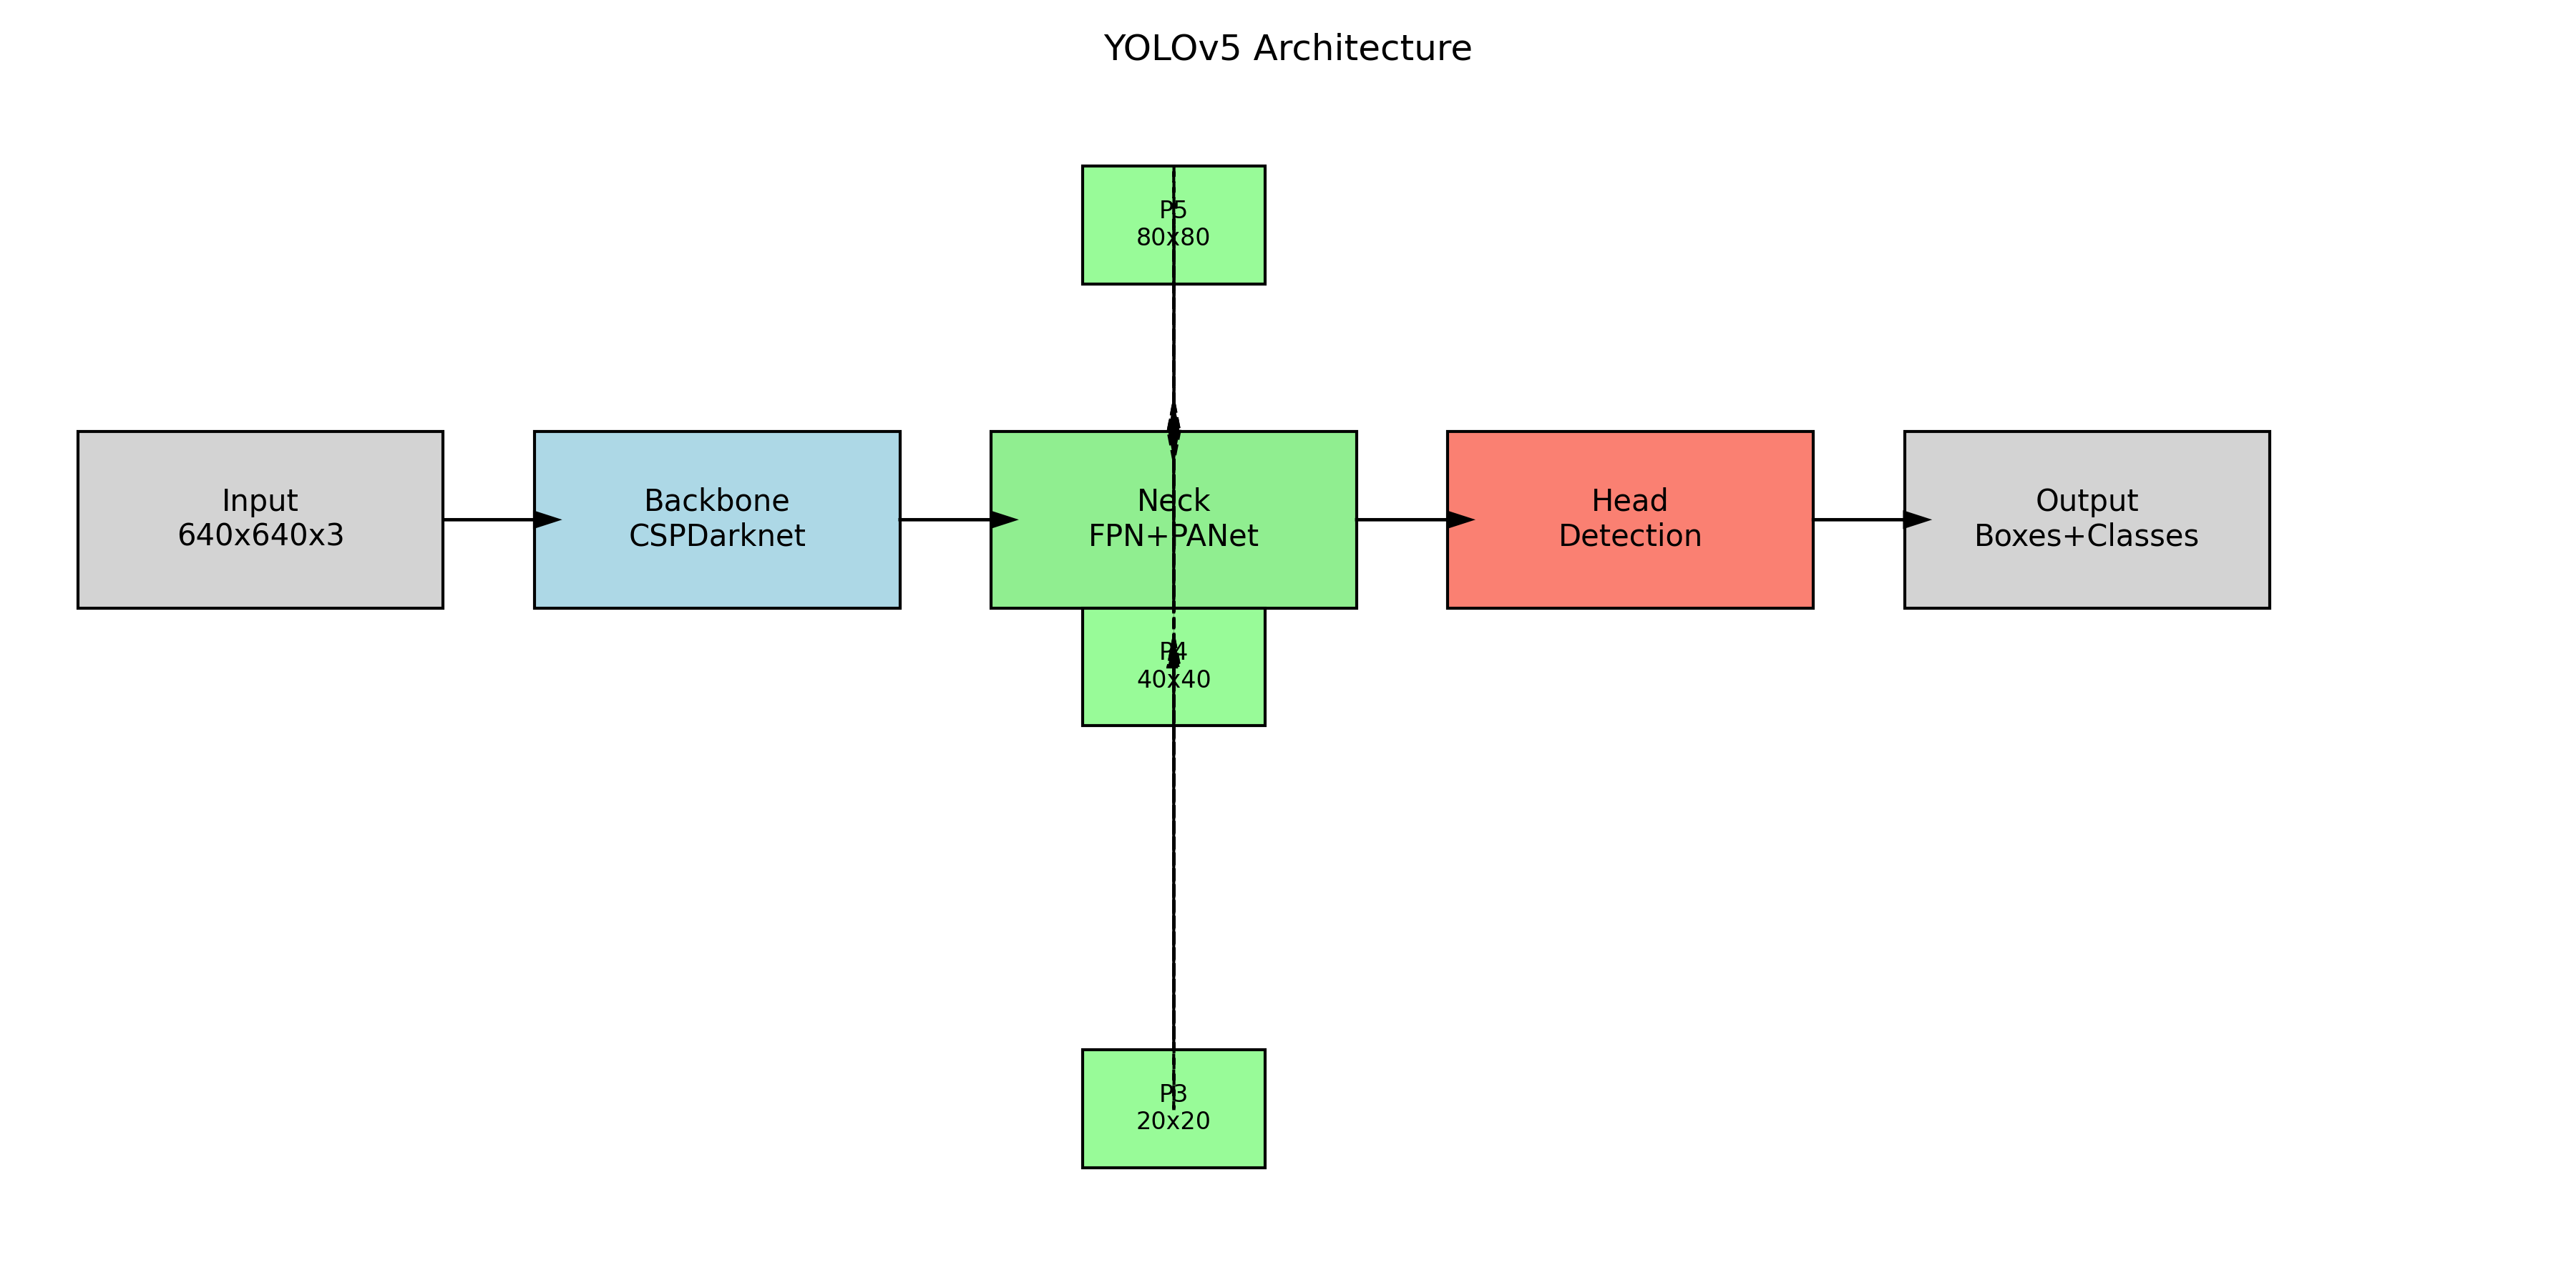
\includegraphics[width=\textwidth]{Dissertation/images/yolov5_architecture.png}
\caption{Схема архитектуры YOLOv5: CSPDarknet backbone (слева), PANet neck (в центре) и трехмасштабная detection head (справа). Цифры указывают количество каналов в слоях. Стрелки показывают направление распространения информации между компонентами.}
\label{fig:yolov5_arch}
\end{figure}

YOLOv5 выпускается в пяти вариантах различного размера (nano, small, medium, large, xlarge), различающихся по количеству параметров и вычислительной сложности. В наших экспериментах используется версия YOLOv5s (small), обеспечивающая хороший баланс между точностью (mAP@0.5: 56.8\%) и скоростью обработки (270 FPS на RTX 4090 в режиме FP16).

\subsection{Модификации YOLOv5 с анти-алиасингом}
\label{methods:yolov5:modifications}

Для улучшения инвариантности YOLOv5 к сдвигам мы разработали две модификации:

\begin{enumerate}
    \item \textbf{AA-YOLOv5} — модель с BlurPool, где все операции даунсэмплинга в backbone заменены на их анти-алиасинговые версии с биномиальным фильтром 3-го порядка. Это включает замену сверточных слоев с шагом 2 на последовательность: свертка с шагом 1 → биномиальный фильтр $[1, 3, 3, 1]/8$ → даунсэмплинг с шагом 2.
    
    \item \textbf{TIPS-YOLOv5} — модель с полифазной выборкой, где операции даунсэмплинга заменены на TIPS-модули с параметрами $(s=2, K=4)$, обеспечивающие явную инвариантность к сдвигам за счет полифазного разложения и адаптивной агрегации компонент.
\end{enumerate}

Оба варианта сохраняют общую структуру исходной модели, изменяя только механизмы даунсэмплинга, что позволяет использовать предобученные веса без необходимости переобучения. Модификации направлены преимущественно на backbone часть сети, поскольку именно эта часть наиболее подвержена проблемам алиасинга из-за множественных операций субдискретизации.

\section{Методология оценки инвариантности}
\label{methods:evaluation}

\subsection{Генерация тестовых последовательностей}
\label{methods:evaluation:sequences}

Для количественной оценки инвариантности к сдвигам мы разработали систему генерации тестовых последовательностей с контролируемыми субпиксельными сдвигами. Каждая последовательность состоит из 32 кадров, где объект (птица) перемещается с шагом 1 пиксель. Точное знание положения объекта на каждом кадре позволяет оценивать стабильность предсказаний при известных сдвигах.

\subsection{Метрики для классификационных моделей}
\label{methods:evaluation:classification}

Для оценки инвариантности классификационных моделей используются следующие метрики:

\begin{itemize}
    \item \textbf{Косинусное сходство} между векторами признаков оригинального и сдвинутого изображений:
    $\rho(x, T_{\delta}x) = \frac{f(x) \cdot f(T_{\delta}x)}{\|f(x)\| \cdot \|f(T_{\delta}x)\|}$
    
    \item \textbf{Дрейф уверенности} — изменение вероятности предсказанного класса при сдвиге:
    $\text{confidence\_drift}(x, T_{\delta}x) = |p_c(x) - p_c(T_{\delta}x)|$
    
    \item \textbf{Стабильность предсказания} — процент кадров в последовательности, на которых модель предсказывает тот же класс, что и на первом кадре.
\end{itemize}

\subsection{Метрики для моделей детекции}
\label{methods:evaluation:detection}

Для оценки инвариантности моделей детекции используются следующие метрики:

\begin{itemize}
    \item \textbf{Средний IoU} между предсказанной ограничивающей рамкой для сдвинутого изображения и скорректированной истинной рамкой с тем же сдвигом.
    
    \item \textbf{Дрейф центра} — расстояние между центром предсказанной рамки и центром истинной рамки в пикселях.
    
    \item \textbf{Стабильность уверенности} — стандартное отклонение значений уверенности детекции по всем кадрам в последовательности.
\end{itemize}

 